\documentclass[11pt,class=report,crop=false]{standalone}
\usepackage[screen]{../exo7book}


\begin{document}

% Commandes spécifiques à ce chapitre

\newcommand{\myvec}[2]{\begin{pmatrix}#1 \\ #2\end{pmatrix}}
\newcommand{\dist}{\text{dist}}

%% Attention les figures sont commentées car longuettes à calculer !!
%\newcommand{\commentfigure}[1]{\centerline{\emph{Ici une figure.}}}  % sans les figures compliquées
\newcommand{\commentfigure}[1]{#1} % avec figures



%====================================================================
\chapitre{Systèmes itérés de fonctions}
%====================================================================


%%%%%%%%%%%%%%%%%%%%%%%%%%%%%%%%%%%%%%%%%%%%%%%%%%%%%%%%%%%%%%%%
\section{Introduction}



Les fractales sont des objets géométriques qui présentent la particularité d'être
\og auto-similaires \fg{}, c'est-à-dire que si l'on zoome sur n'importe quelle partie de l'objet, alors on retrouve
presque l'objet initial. Il est plus simple de prendre un exemple : le flocon de Koch.

\commentfigure{
\myfigure{1}{\tikzinput{fig_ifs-koch01}}
}


En inspectant cette figure, on s'aperçoit de cette propriété d'auto-similarité.
Cela devient beaucoup plus clair si l'on sait comment cette figure a été construite.

On part d'un segment horizontal de longueur $1$. Nous réduisons ce segment d'un facteur $3$
et produisons $4$ copies de ce petit segment. Ces $4$ copies forment maintenant une dent.
Partons de cette dent, effectuons une réduction d'un facteur $3$, et produisons $4$ petites dents...
On itère le processus indéfiniment et la \og limite \fg{} est notre flocon de Koch.

\bigskip


\commentfigure{
\myfigure{1}{\tikzinput{fig_ifs-koch02}}
}


C'est un objet \og fractal \fg{} différent des figures géométriques classiques. Il possède des propriétés 
surprenantes. Essayez par exemple de deviner quelle est sa longueur. Nous calculerons aussi sa dimension, et nous constaterons que ce n'est pas une courbe lisse (de dimension $1$), ni une surface (de dimension $2$), mais un objet intermédiaire !
Ce qui est aussi fascinant, c'est qu'avec des transformations extrêmement simples on arrive à fabriquer
des objets d'une complexité et d'une beauté infinies.

La seconde motivation de ce chapitre est la mise en pratique des transformations usuelles du plan :
translations, réflexions, rotations, homothéties et plus généralement des transformations affines.
L'usage des matrices facilite grandement la manipulation de ces applications.


%%%%%%%%%%%%%%%%%%%%%%%%%%%%%%%%%%%%%%%%%%%%%%%%%%%%%%%%%%%%%%%%
\section{Topologie de $\Rr^2$}

%---------------------------------------------------------------
\subsection{Distance}

Nous choisissons comme distance la \defi{distance euclidienne} : si $P(x,y)$
et $Q(x',y')$ sont deux points du plan $\Rr^2$, alors la distance entre 
$P$ et $Q$ est
$$\| P - Q\| = \sqrt{(x-x')^2+(y-y')^2}.$$
C'est bien sûr la distance associée à la \defi{norme euclidienne} :
$$\|(x,y)\| = \sqrt{x^2+y^2}.$$

Une \defi{isométrie} est une application $f : \Rr^2 \to \Rr^2$ qui
préserve les distances, c'est-à-dire :
$$\forall P,Q \in \Rr^2 \quad \|f(P)-f(Q)\| = \|P-Q\|.$$
Nous démontrerons plus loin que les translations, rotations et réflexions sont des isométries.
Par contre, une homothétie de rapport $k\neq +1,-1$ n'est pas une isométrie.


Pour un réel $k\ge 0$, une application $f$ est dite \defi{lipschitzienne de rapport $k$}
si 
$$\forall P,Q \in\Rr^2 \quad \|f(P)-f(Q)\| \le k \|P-Q\|.$$
Par exemple,  une isométrie est lipschitzienne de rapport $1$,
une homothétie de rapport $k\ge 0$
est lipschitzienne de rapport $k$.

Les applications dont nous aurons besoin devront réduire les distances:
une application $f$ est dite \defi{contractante} (ou est une \defi{contraction}) s'il existe $0 \le k<1$
telle que 
$$\forall P,Q \in\Rr^2 \quad \|f(P)-f(Q)\| \le k \|P-Q\|.$$
Autrement dit, une application est contractante si et seulement si elle est lipschitzienne
pour un rapport $k<1$.

%---------------------------------------------------------------
\subsection{Compacts de $\Rr^2$}

Voici des rappels.

\begin{itemize}
  \item Un ensemble $F\subset \Rr^2$ est un \defi{fermé} si, pour toute suite de points $(P_n)_{n\in\Nn}$
telle que $P_n \in F$ (pour tout $n$) et $P_n \to Q$, on a $Q\in F$.
  \item Un ensemble $O \subset \Rr^2$ est un \defi{ouvert} si $\Rr^2 \setminus O$ est un fermé.
  \item Un ensemble est \defi{borné} s'il est inclus dans un disque. 
Autrement dit, $B \subset \Rr^2$  est borné s'il existe un $R>0$ tel que $B \subset D(O,R)$, où
on a noté $D(O,R)$ le disque fermé de centre $O$ et de rayon $R$.
  \item Un ensemble sera appelé un \defi{compact} s'il est fermé et borné.
  \item Exemple : $[a,b] \times [c,d]$ est un compact de $\Rr^2$.
\end{itemize}


\begin{theoreme}
\label{th:intersectioncompacts}
Soit $\{ C_n\}_{n\in \Nn}$ une famille de compacts non vides de $\Rr^2$.
Si $C_0 \supset C_1 \supset C_2 \supset C_3 \supset \cdots$, alors 
$$C = \bigcap_{n\ge0} C_n$$
est un compact non vide de $\Rr^2$.
\end{theoreme}

%\commentfigure{
\myfigure{1}{\tikzinput{fig_ifs13}}
%}


Remarquez que, vu l’emboîtement des compacts, alors on a en fait
$C_0\cap C_1=C_1$, $C_0\cap C_1\cap C_2=C_2$,\ldots
Et donc, en d'autres termes, le théorème affirme qu'une famille de compacts emboîtés
tend vers un compact.

\bigskip

Voici le résultat fondamental concernant les fonctions continues sur les ensembles compacts. Le premier
point est pour une fonction à valeurs dans $\Rr$, le second point est sa version pour une fonction à valeurs dans $\Rr^2$.
\begin{theoreme}
\sauteligne
\begin{enumerate}
  \item Une fonction continue sur un compact est bornée et atteint ses bornes.
Autrement dit, si $C \subset \Rr^2$ est un ensemble compact et  $f : C  \to \Rr$ est une fonction continue,
alors :
  \begin{itemize}
    \item d'une part la fonction est bornée, 
    \item et d'autre part le maximum et le minimum de $f$ sont atteints en des points de $C$.
  \end{itemize}
 
  \item Soit $C \subset \Rr^2$ un ensemble compact et soit $f : C  \to \Rr^2$ une fonction continue.
Alors $f(C)$ est un ensemble compact de $\Rr^2$.
\end{enumerate}
\end{theoreme}


%---------------------------------------------------------------
\subsection{Distance de Hausdorff}
\label{ssec:haus}

Pour $E \subset \Rr^2$ et $r \ge 0$, notons 
$$E(r) = \big\{ P \in \Rr^2 \mid \| P - Q \| \le r \text{ pour un } Q \in E \big\}$$
le \defi{$r$-voisinage} de $E$.
C'est l'ensemble des points situés dans $E$ ou à une distance inférieure à $r$ de $E$.
Sur la figure ci-dessous, $E$ est l'ensemble gris foncé, alors que $E(r)$ est l'ensemble des points en gris clair et gris foncé.

%\commentfigure{
\myfigure{0.9}{\tikzinput{fig_ifs14}}
%}


La \defi{distance de Hausdorff} entre deux ensembles $E, F \subset \Rr^2$
est
$$\dist_H(E,F) = \inf \big\{ r \ge 0 \mid F \subset E(r) \text{ et } E \subset F(r) \big\}.$$
C'est donc la plus petite valeur de $r$ telle que $F$ est inclus dans le $r$-voisinage de $E$,
et $E$ dans le $r$-voisinage de $F$.


Sur le dessin suivant, on considère $E$ et $F$ deux ellipses (avec les points intérieurs). On a trouvé le plus 
petit $r_1$ tel que $F \subset E(r_1)$, c'est-à-dire que l'on a fait grossir l'ellipse pleine $E$ jusqu'à ce qu'elle contienne $F$. Et $r_2$ est le plus petit réel tel que $E \subset F(r_2)$. La distance de Hausdorff entre $E$ et $F$ est le minimum entre $r_1$ et $r_2$.

%\commentfigure{
\myfigure{1}{\tikzinput{fig_ifs15}}
%}


Cela n'a rien à voir avec la distance usuelle entre deux ensembles (le distance la plus courte pour aller 
de l'un à l'autre).

\begin{proposition}
\label{prop:haus}
Sur l'ensemble $\mathcal{C}$ de tous les compacts de $\Rr^2$, $\dist_H$ définit une distance. Autrement dit, pour tous $E,F,G \in \mathcal{C}$ :
\begin{enumerate}
  \item $\dist_H(E,F)=0$ si et seulement si $E=F$,

  \item $\dist_H(E,F)=\dist_H(F,E)$,

  \item $\dist_H(E,G) \le \dist_H(E,F)+\dist_H(F,G)$.
\end{enumerate}

\end{proposition}

\begin{proof}
Pour la première propriété: 
si $E=F$, alors $E \subset F(0)$ (comme $F$ est une partie fermée, $F(0)=F$ est le $0$-voisinage de $F$) et $F \subset E(0)$, donc $\dist_H(E,F)=0$.
Réciproquement, supposons que $E \neq F$ et montrons que $\dist_H(E,F)>0$.
Comme $E\neq F$, supposons par exemple que $F$ n'est pas inclus dans $E$, c'est-à-dire qu'il existe $P\in F$ tel que $P\notin E$.
Si l'on note $r$ la distance entre $P$ et $E$ (ici il s'agit de la distance
usuelle entre un point et un ensemble : $d(P,E)=\inf\{ \|P-Q\| \mid Q \in E\}$),
alors $P \notin E(\frac r 2)$ et donc $\dist_H(E,F) \ge \frac r2 >0$.

La deuxième propriété est évidente, et la troisième se déduit 
de l'inégalité triangulaire pour la distance entre deux points (voir l'exercice \ref{exo:ifs2}).
\end{proof}


%%%%%%%%%%%%%%%%%%%%%%%%%%%%%%%%%%%%%%%%%%%%%%%%%%%%%%%%%%%%%%%%
\section{Attracteurs}

Soient $f_i : \Rr^2 \to \Rr^2$ des fonctions, $i=1,\ldots,\ell$. 
Soit $E \subset \Rr^2$ un ensemble.
Rappelons que l'\defi{image directe} de $E$ par $f_i$ est
$$f_i(E) =\big\{ f_i(x,y) \mid (x,y) \in E \big\}.$$
Nous allons généraliser cette notion à une famille de fonctions. 
L'\defi{image directe} de la famille 
$\mathbf{f}=\{f_i\}_{i=1,\ldots,\ell}$ est :
$$\mathbf{f}(E) = \bigcup_{i=1}^{\ell} f_i(E).$$

Si $E$ est une partie compacte et que les $f_i$ sont continues, alors $f_i(E)$
et $\mathbf{f}(E)$ sont aussi des parties compactes de $\Rr^2$.
On note $f_i^2(E) = f_i(f_i(E))$, $f_i^3(E) = f_i(f_i(f_i(E)))$,...
et plus généralement $f_i^{k+1}(E) = f_i \big(f_i^k(E)\big)$.
De même, pour notre famille, on définit par récurrence
 $\mathbf{f}^{k+1}(E) = \mathbf{f} \big( \mathbf{f}^k(E)\big)$.

%---------------------------------------------------------------
\subsection{Le théorème d'attraction}


\begin{theoreme}
\label{th:attraction}
Soit $f_i : \Rr^2 \to \Rr^2$, $i=1,\ldots,\ell$, une famille de contractions.
Alors il existe un unique compact non vide $C \subset \Rr^2$ qui est invariant par la famille
$\mathbf{f} = \{f_i\}$ :
$$C= \mathbf{f}(C),$$
c'est-à-dire 
$$C = \bigcup_{i=1}^{\ell} f_i(C).$$

De plus, pour toute partie compacte non vide $E \subset \Rr^2$ telle que 
$\mathbf{f}(E) \subset E$ (c'est-à-dire $f_i(E) \subset E$, $i=1,\ldots,\ell$),
la suite des itérés 
$\mathbf{f}^k(E)$ converge vers $C$:
$$C = \bigcap_{k=1}^{+\infty} \mathbf{f}^k(E).$$
\end{theoreme}



L'ensemble $C$ obtenu est l'\defi{attracteur} de la famille
$\mathbf{f}=\{f_i\}$.

\begin{remarque*}
\sauteligne
\begin{itemize}

 \item La première partie de ce théorème est un résultat théorique d'existence et d'unicité ;
la seconde partie est un résultat pratique qui permet de calculer l'attracteur.


  \item Remarquez que, comme les ensembles $\mathbf{f}^k(E)$ vont être emboîtés, 
alors prendre cette intersection infinie n'est juste qu'une façon rigoureuse d'écrire la limite de $\mathbf{f}^k(E)$ quand $k\to +\infty$.

 \item Si les $f_i$ ne sont pas des contractions, le théorème n'est plus valide. Par exemple,
imaginez que les $f_i$ soient des translations.
\end{itemize}
\end{remarque*}

\bigskip

Il existe une version améliorée de la deuxième partie du théorème d'attraction.
Dans cet énoncé, on se débarrasse de l'hypothèse $\mathbf{f}(E) \subset E$ : ainsi 
$E$ est une partie compacte non vide quelconque. 

\begin{theoreme}
\label{th:attractionbis}
Avec les notations du théorème \ref{th:attraction} :
soit $E$ une partie compacte non vide de $\Rr^2$. Alors 
la suite des itérés $\mathbf{f}^k(E)$ converge vers $C$:
$$C = \lim_{k\to+\infty} \mathbf{f}^k(E).$$
\end{theoreme}

\begin{remarque*}
\sauteligne
\begin{itemize}
  \item Nous admettons ce théorème, qui est en fait un résultat vrai dans le cadre général des espaces complets.
  
  \item On peut prendre comme ensemble $E$ un seul point ! C'est ce que nous ferons
  dans la section \ref{ssec:chaos} pour tracer efficacement nos fractales.
  
  \item Vous connaissez déjà ce théorème dans sa version simple. En effet, si l'on considère une famille composée d'une seule fonction contractante $f : \Rr \to \Rr$,
alors on sait que notre fonction admet un unique point fixe $c\in \Rr$. Notre attracteur est ici $C=\{c\}$.
De plus $c$ s'obtient comme la limite d'une suite récurrente: partant de n'importe quel $x_0 \in \Rr$,
la suite $(x_k)$ définie par $x_{k}= f(x_{k-1})$ (autrement dit $x_k = f^k(x_0)$) converge vers $c$.
\end{itemize}
\end{remarque*}


%---------------------------------------------------------------
\subsection{L'ensemble de Cantor}


Nous illustrons ce théorème par un exemple simple, 
non pas du plan, mais de la droite.
Considérons les deux fonctions
$$f_1(x)=\frac 13x, \qquad f_2(x)=\frac 23 + \frac 13x.$$
La famille $\mathbf{f}=\{f_1,f_2\}$ est constituée d'applications 
de $\Rr$ dans $\Rr$ contractantes (elles sont toutes deux
lipschitziennes de rapport $k=\frac 13$).

\commentfigure{
\myfigure{1}{\tikzinput{fig_ifs-cantor01}}
}

Soit $C_0$ le segment $[0,1] \subset \Rr$. Alors
$f_1(C_0)=[0,\frac 13]$ et $f_2(C_0) = [\frac 23, 1]$.
Donc $C_1 = \mathbf{f}(C_0) = f_1(C_0)\cup f_2(C_0) = [0,\frac 13] \cup [\frac 23, 1]$. Noter que $\mathbf{f}(C_0) \subset C_0$.
Au cran suivant :
$f_1(C_1) = [0,\frac 19] \cup [\frac 29,\frac 39]$
et $f_2(C_1) = [\frac69,\frac 79] \cup [\frac 89,\frac 99]$.
Donc $C_2 = \mathbf{f}(C_1) = f_1(C_1) \cup f_2(C_1)$ est l'union de $4$ segments.
On itère le processus :
$C_n= \mathbf{f}(C_{n-1})$ est l'union de $2^n$ segments, 
chaque segment étant de longueur $\frac{1}{3^n}$.

Une autre façon de décrire le processus est que, à chaque étape,
on divise chaque segment en trois et on retire celui du milieu.
L'attracteur $C$ obtenu est l'\defi{ensemble de Cantor}, appelé
aussi joliment les \defi{poussières de Cantor}.
L'ensemble obtenu n'est pas vide ; il est même non dénombrable !


%---------------------------------------------------------------
\subsection{Preuve}

Passons à la preuve du théorème \ref{th:attraction} d'attraction.

\textbf{Existence de l'attracteur.}
Comme les $f_i$ sont des contractions, il existe un disque fermé $D= D(O,r)$
(centré à l'origine $O$ et de rayon $r$ assez grand) tel que
$f_i(D) \subset D$ pour tout $i=1,\ldots,\ell$.
En effet, en notant $k_i$ le rapport de contraction de $f_i$ et 
$a_i = \| f_i(O) \|$ pour tout $i = 1,\ldots,\ell$,
puis $k = \max_{i=1,\ldots,\ell} k_i$
et $a = \max_{i=1,\ldots,\ell} a_i$, 
on a $0 \le k < 1$ et $a \ge 0$.
Puisque $f_i$ est une contraction, on en déduit que, pour tout $x \in D$,
$$\| f_i(x)-f_i(O) \| \le k_i \| x \| \le kr
\quad \text{ et donc } \quad
\| f_i(x) \| \le kr+a.$$
Ainsi, 
$$\text{ si } \quad  r \ge \frac{a}{1-k}, \quad \text{ alors } \quad \| f_i(x) \| \le r.$$
En d'autres termes, $\mathbf{f}(D) \subset D$.
En composant par $\mathbf{f}$, cela implique $\mathbf{f}\left(\mathbf{f}(D) \right) \subset \mathbf{f}(D)$,
donc $\mathbf{f}^2(D) \subset \mathbf{f}^1(D)$
et par récurrence $\mathbf{f}^{k+1}(D) \subset \mathbf{f}^k(D)$.

\medskip

L'ensemble de départ $D$ est un fermé borné de $\Rr^2$ donc un compact.
Les applications $f_i$ sont contractantes donc continues, ainsi
les $f_i(D)$ sont des compacts et $\mathbf{f}(D)$ également, de même pour $\mathbf{f}^k(D)$.
Donc  $\left(\mathbf{f}^k(D)\right)_k$ est une suite de compacts non vides,
décroissante pour l'inclusion. Alors $C = \bigcap_{k=1}^{+\infty} \mathbf{f}^k(D)$
est un ensemble compact non vide d'après le théorème \ref{th:intersectioncompacts}. 
Noter encore une fois que, comme les ensembles $\mathbf{f}^k(D)$ sont emboîtés, 
prendre cette intersection infinie n'est juste qu'une façon rigoureuse d'écrire
la limite de $\mathbf{f}^k(D)$ quand $k\to +\infty$. 

Nous allons maintenant montrer que $C$ est un ensemble fixé par nos transformations, c'est-à-dire
$\mathbf{f}(C)=C$.
Notons $D_k = \mathbf{f}^k(D)$, autrement dit $D_0 = D$ et $D_{k+1} = \mathbf{f}(D_k)$. Ainsi
$(D_k)$ est notre suite de compacts emboîtés et $\bigcap_{k=1}^{+\infty} D_k = C$.


\begin{itemize}
  \item Preuve de $\mathbf{f}(C) \subset C$.  
  Soit $y \in \mathbf{f}(C)$. Alors 
  $$y \in \mathbf{f}\left(\bigcap_{k=1}^{+\infty} D_k\right)
  \quad \text{ donc, pour tout $k\ge 1$, } y \in \mathbf{f}(D_k).$$
   Ainsi
  $$y \in \bigcap_{k=1}^{+\infty}\mathbf{f}(D_k) 
  = \bigcap_{k=1}^{+\infty} D_{k+1} = \bigcap_{k=2}^{+\infty} D_{k}
  = \bigcap_{k=1}^{+\infty} D_{k} = C.$$
  
  \item Preuve de $C \subset \mathbf{f}(C)$.
  Soit $y \in C$. Alors, pour tout $k\ge1$, $y \in D_k$.
  Donc, pour tout $k\ge0$, $y \in D_{k+1}$. Ainsi, 
  pour tout $k\ge0$, $y \in \mathbf{f}({D_k})$.
  
  Pour chaque $k\ge0$, il existe donc $x_k \in D_k$ tel que 
  %$y \in \mathbf{f}({x_k})$, c'est-à-dire 
  $y = f_i(x_k)$, pour un certain $1 \le i \le \ell$ (ce $i$ dépend de $k$).
  Les $x_k$ sont tous dans le compact $D$. Donc on peut extraire une sous-suite $(x_{\varphi(k)})$ 
  qui converge vers $x_\infty \in D$. 
  Il n'est pas dur de montrer qu'en fait $x_\infty$ appartient à $C$. En effet,
  les $x_{\varphi(k)}$ sont dans le fermé $D_{k_0}$ pour tout $k\ge k_0 \ge 1$, donc la limite 
  $x_\infty$ est aussi dans $D_{k_0}$. Comme c'est vrai quel que soit $k_0$, alors $x_\infty \in C$.
  
  Pour chaque $k$, il n'existe qu'un nombre fini de choix possibles pour le $i$
  tel que $y = f_i(x_{\varphi(k)})$. Quitte à extraire de nouveau une sous-suite de $(x_{\varphi(k)})$,
  on peut supposer que $y = f_{i_0}(x_{\varphi(k)})$
  pour tout $k\ge0$, pour un certain $1 \le i_0 \le \ell$. La fonction $f_{i_0}$ est une contraction donc continue, ainsi à la limite on a encore
  $y = f_{i_0}(x_\infty)$. Ainsi $y \in f_{i_0}(C)$ et donc $y \in \mathbf{f}(C)$.
   
\end{itemize}

Conclusion :  $\mathbf{f}(C) = C$.

%Comme à chaque étape $\mathbf{f}\left(\mathbf{f}^k(D)\right) \subset \mathbf{f}^k(D)$
%alors  $\mathbf{f}\left(\bigcap_{k=1}^{+\infty} \mathbf{f}^{k}(D)\right) 
%= \bigcap_{k=1}^{+\infty} \mathbf{f}^{k+1}(D) = \bigcap_{k=2}^{+\infty} \mathbf{f}^{k}(D) =
%\bigcap_{k=1}^{+\infty} \mathbf{f}^{k}(D) = C$ donc $\mathbf{f}(C) = C$.

Ce que nous venons de faire pour le disque $D$ fonctionne pour n'importe quelle partie
compacte non vide $E$ telle que $\mathbf{f}(E) \subset E$. Nous avons donc aussi 
prouvé la seconde partie du théorème.

\bigskip

\textbf{Unicité.}
Nous allons utiliser la distance de Hausdorff introduite plus haut (paragraphe \ref{ssec:haus}).
En effet, si $f_i$ est contractante de rapport $k_i < 1$ alors, pour deux compacts
$C,C' \subset \Rr^2$, nous avons 
$\dist_H (f_i(C),f_i(C')) \le k_i \cdot \dist_H (C,C')$ (voir l'exercice \ref{exo:ifs2}).
En notant encore $k = \max_{i=1,\ldots,\ell} k_i$, on a donc $0 \le k < 1$ et 
$\dist_H (\mathbf{f}(C),\mathbf{f}(C')) \le  k  \cdot  \dist_H (C,C')$.

Supposons que $C$ et $C'$ soient deux compacts invariants : $\mathbf{f}(C) = C$ et
$\mathbf{f}(C') = C'$. Alors $\dist_H (C,C') \le k  \cdot  \dist_H (C,C')$.
Comme $k < 1$, alors $\dist_H (C,C')=0$ et donc, par la proposition \ref{prop:haus},
$C=C'$.


%%%%%%%%%%%%%%%%%%%%%%%%%%%%%%%%%%%%%%%%%%%%%%%%%%%%%%%%%%%%%%%%
\section{Isométries, similitudes}

Nous allons étudier quelques transformations élémentaires du plan.

%---------------------------------------------------------------
\subsection{Transformations élémentaires}

% L'image originale du Shadok !
% \tikzinput{fig_ifs01}


\subsubsection*{Translations.}
Notons $\myvec{e}{f}$ un élément de $\Rr^2$.
La \defi{translation de vecteur $\myvec{e}{f}$} est l'application 
de $\Rr^2$ dans $\Rr^2$ définie par
$$\myvec{x}{y} \mapsto \myvec{x}{y} + \myvec{e}{f}.$$

%\commentfigure{
\myfigure{1}{\tikzinput{fig_ifs02}}
%}


\subsubsection*{Rotations.}
La \defi{rotation} de centre l'origine et d'angle $\theta$
est l'application de $\Rr^2$ dans $\Rr^2$ définie par
$$\myvec{x}{y} \mapsto \myvec{x \cos \theta - y \sin \theta}{x\sin \theta + y \cos \theta}.$$

\`A ce point, il est plus facile d'utiliser l'écriture matricielle :
$$\myvec{x}{y} \mapsto \begin{pmatrix}\cos \theta & -\sin \theta \\ 
\sin\theta & \cos \theta\\ \end{pmatrix}\myvec{x}{y}.$$

%\commentfigure{
\myfigure{1}{\tikzinput{fig_ifs03}}
%}

On notera $M_\theta$ la matrice de la rotation d'angle $\theta$:
$$M_\theta = \begin{pmatrix}\cos \theta & -\sin \theta \\ 
\sin\theta & \cos \theta\\ \end{pmatrix}.$$

\subsubsection*{Homothéties.}
L'\defi{homothétie} de centre l'origine et de rapport $k \in \Rr\setminus\{0\}$ est l'application 
de $\Rr^2$ dans lui-même définie par :
$$\myvec{x}{y} \mapsto \myvec{kx}{ky}.$$
Notez que $\myvec{kx}{ky}$ peut aussi s'écrire $k\myvec{x}{y}$.

%\commentfigure{
\myfigure{1}{\tikzinput{fig_ifs04}}
%}

\subsubsection*{Réflexions.}
Nous commençons par regarder la réflexion par rapport à l'axe des abscisses :
c'est l'application de $\Rr^2$ dans $\Rr^2$ définie par
$$\myvec{x}{y} \mapsto \myvec{x}{-y}.$$
En termes de matrice, l'écriture est la suivante :
$$\myvec{x}{y} \mapsto \begin{pmatrix}1 & 0 \\ 0 & -1\end{pmatrix}\myvec{x}{y}.$$

Plus généralement l'expression d'une réflexion par rapport à un axe passant par l'origine et faisant un angle $\frac\theta2$ avec l'axe des abscisses est
$$\myvec{x}{y} \mapsto \begin{pmatrix}\cos \theta & \sin \theta \\ 
\sin\theta & -\cos \theta\\ \end{pmatrix}\myvec{x}{y}.$$

%\commentfigure{
\myfigure{1}{\tikzinput{fig_ifs05}}
%}


%---------------------------------------------------------------
\subsection{Similitudes}

\`A partir de ces transformations élémentaires, nous pouvons en inventer de nouvelles.
Ce qui est remarquable, c'est qu'en composant un nombre quelconque de translations,
rotations, homothéties et réflexions, la fonction qui en résulte est l'une des deux suivantes :

\subsubsection*{Similitude directe.}
C'est une application de $\Rr^2$ dans lui-même définie 
par
$$\myvec{x}{y} \mapsto k\begin{pmatrix}\cos \theta & -\sin \theta \\ 
\sin\theta & \cos \theta\\ \end{pmatrix}\myvec{x}{y} + \myvec{e}{f},$$
où $k > 0$, $\theta \in[0,2\pi[$, $e, f \in \Rr$.
C'est donc la composée d'une homothétie, d'une rotation et d'une translation.


\subsubsection*{Similitude indirecte.}
C'est une application de $\Rr^2$ dans lui-même définie 
par
$$\myvec{x}{y} \mapsto k\begin{pmatrix}\cos \theta & \sin \theta \\ 
\sin\theta & -\cos \theta\\ \end{pmatrix}\myvec{x}{y} + \myvec{e}{f},$$
où $k > 0$, $\theta \in[0,2\pi[$, $e, f \in \Rr$.
C'est la composée d'une homothétie, d'une réflexion et d'une translation.




Ce qui va nous intéresser ici est la chose suivante :
\begin{proposition}
\sauteligne
\begin{enumerate}
 \item Les translations, rotations et réflexions conservent les distances (ce sont des isométries).
 \item Une homothétie de rapport $k$ multiplie les distances d'un facteur $|k|$.
 \item Une similitude est contractante si et seulement si son rapport 
vérifie $0 < k < 1$.
 \item La composition de similitudes contractantes est une similitude contractante.
\end{enumerate}
\end{proposition}

\begin{proof}~
\begin{enumerate}
 \item \begin{itemize}
        \item Si $g$ est une translation de vecteur $(e,f)$, notons $P(x,y)$ et $Q(x',y')$ deux points du plan.
Alors $g(P)-g(Q)=g(x,y)-g(x',y') = (x+e,y+f)-(x'+e,y'+f)=(x,y)-(x',y')=P-Q$,
donc en particulier  pour les distances $\|g(P)-g(Q)\| = \|P-Q\|$, ce qui en fait une isométrie.
  
        \item Pour montrer qu'une application linéaire $g$ est une isométrie, il suffit de montrer que 
\begin{equation}
\label{eq:iso}
\forall (x,y) \in \Rr^2 \quad \| g(x,y) \| = \| (x,y) \|.
\end{equation}
C'est-à-dire que l'on regarde seulement la distance entre les points et l'origine.
En effet, si (\ref{eq:iso}) est vraie, alors pour tous $(x,y), (x',y')$ nous obtenons
$\|g(x,y)-g(x',y')\| = \|g(x-x',y-y')\|=\|(x-x',y-y')\|=\|(x,y)-(x',y')\|$
(la linéarité joue un rôle essentiel).

Appliquons ceci à une rotation d'angle $\theta$,
$g(x,y)= (x \cos \theta - y \sin \theta,x\sin \theta + y \cos \theta)$.
Donc $\|g(x,y) \|^2 = (x \cos \theta - y \sin \theta)^2 + (x\sin \theta + y \cos \theta)^2=
x^2+y^2= \| (x,y) \|^2$. (On utilise le fait que $\cos^2\theta + \sin^2\theta=1$.)

        \item Pour une réflexion, les calculs sont similaires. 
       \end{itemize}


 \item On peut supposer que le centre de l'homothétie est à l'origine. 
L'expression de $g$ est alors $g(x,y)=(kx,ky)$ et donc 
$\|g(x,y) \| = |k| \cdot  \|(x,y)\|.$

 \item Une similitude de rapport $k > 0$ est la composition d'isométries et d'une 
homothétie de rapport $k$. Elle est donc contractante si et seulement si l'homothétie l'est.

 \item Ce point découle du fait qu'une similitude de rapport $k$ composée avec une similitude de rapport $k'$ est une similitude de rapport $k\cdot k'$. 
\end{enumerate}
\end{proof}




\begin{proposition}
L'ensemble des similitudes (directes ou indirectes) forme un groupe pour la composition.
\end{proposition}

\begin{proof}
\`A faire en exercice !
\end{proof}

Exercice : écrire toutes les transformations précédentes à l'aide des nombres complexes.
Par exemple l'application $z \mapsto e^{\ii \theta} z$ est la rotation d'angle 
$\theta$, centrée à l'origine. 


%%%%%%%%%%%%%%%%%%%%%%%%%%%%%%%%%%%%%%%%%%%%%%%%%%%%%%%%%%%%%%%%
\section{Exemples à partir de similitudes}

Nous avons déjà vu l'ensemble de Cantor. 
Reprenons maintenant l'exemple introductif à ce chapitre.


%---------------------------------------------------------------
\subsection{Le flocon de Koch}


Soient les transformations affines suivantes :
$$f_1 \myvec{x}{y} = \frac13 \myvec{x}{y} \qquad \qquad
f_2\myvec{x}{y} = \frac13 M_{\frac \pi 3} \myvec{x}{y}+ \myvec{\frac13}{0}$$
$$f_3\myvec{x}{y} = \frac13 M_{-\frac \pi 3}\myvec{x}{y}+ \myvec{\frac12}{\frac{\sqrt 3}{6}} \qquad \qquad
f_4\myvec{x}{y} = \frac13 \myvec{x}{y}+ \myvec{\frac23}{0}$$

Ce sont toutes des similitudes de rapport $\frac 13$.
Rappelons que $M_\theta = \begin{pmatrix}\cos \theta & -\sin \theta \\ 
\sin\theta & \cos \theta\\ \end{pmatrix}$
est la matrice de la rotation d'angle $\theta$.
Chacune de ces transformations envoie le segment $K_0 = [0,1]\times \{0\}$
sur un petit segment. (Le petit triangle rouge sert seulement ici à distinguer
le \og haut \fg{} du \og bas \fg{}.) On a représenté $K_0,\ldots,K_4$.

\commentfigure{
\myfigure{1}{\tikzinput{fig_ifs-koch03}}
}

$K_1$ est donc la figure composée d'une seule \og dent \fg{}. L'attracteur obtenu en itérant le processus indéfiniment est le flocon de Koch. (On applique ici le théorème \ref{th:attractionbis}, car 
on n'a pas $\mathbf{f}(K_0) \subset K_0$.)
En fait, pour obtenir un vrai flocon, il faut réunir trois attracteurs.
\commentfigure{
\myfigure{1}{\tikzinput{fig_ifs-koch04}}
}


%---------------------------------------------------------------
\subsection{Le triangle de Sierpinski}

On part de $S_0$ le triangle équilatéral dont les sommets sont $(0,0)$,
$(1,0)$, $(\frac12,\frac{\sqrt3}{2})$. On considère les trois transformations affines suivantes :
$$f_1 \myvec{x}{y} = \frac12 \myvec{x}{y} \qquad
f_2\myvec{x}{y} = \frac12 \myvec{x}{y}+ \myvec{\frac12}{0} \qquad
f_3\myvec{x}{y} = \frac12 \myvec{x}{y}+ \myvec{\frac14}{\frac{\sqrt3}{4}}
$$

Chacune des transformations $f_i$ est la composition d'une homothétie de rapport $\frac12$ et d'une translation.
\`A la première étape, chacune envoie donc le grand triangle équilatéral $S_0$ sur un triangle plus petit.
Géométriquement, on retire des triangles au centre de chaque plus gros triangle.
On a représenté $S_0$, $S_1$, $S_2$, $S_3$ et $S_6$, ce qui donne une bonne idée
de l'attracteur, appelé le \defi{triangle de Sierpinski}.

\commentfigure{
\myfigure{1}{\tikzinput{fig_ifs-sierp01}}
}


%---------------------------------------------------------------
\subsection{D'autres fractales}

Il est possible de construire bien d'autres figures : voici par exemple le flocon de Koch à $85^\circ$. Il y a aussi le tapis de Sierpinski, et en trois dimensions l'éponge de Sierpinski... \`A vous d'en découvrir d'autres !
\commentfigure{
\myfigure{1}{\tikzinput{fig_ifs-koch-85}}
}




%%%%%%%%%%%%%%%%%%%%%%%%%%%%%%%%%%%%%%%%%%%%%%%%%%%%%%%%%%%%%%%%
\section{Transformations affines}

%---------------------------------------------------------------
\subsection{Définition}

Une \defi{transformation affine} du plan est une application
de $\Rr^2$ dans lui-même définie 
par
$$\myvec{x}{y} \mapsto \begin{pmatrix}a & b \\ c & d \\  \end{pmatrix}
\myvec{x}{y} + \myvec{e}{f},$$
où $a,b,c,d, e, f$ sont des réels quelconques.

En d'autres termes, à un point $(x,y)$ du plan
on associe le point $(x',y')$ défini par 
$$\left \{
\begin{array}{rcl}
    x' &=& ax + by + e \\
    y' &=& cx + dy + f \\
\end{array}
\right..$$

En fait, une transformation affine $f$ est la composée d'une transformation
linéaire $g$ et d'une translation $t$ : $f = t \circ g$.
Ici la transformation linéaire est l'application :
$$\myvec{x}{y} \mapsto \begin{pmatrix}a & b \\ c & d \\  \end{pmatrix}
\myvec{x}{y}.$$


%---------------------------------------------------------------
\subsection{Exemples}

Bien sûr, les translations, rotations, réflexions, homothéties et similitudes sont
des transformations affines. Mais voici de nouveaux exemples.

\subsubsection*{Exemple général}

Oublions la translation et concentrons-nous sur l'application $f$ définie par
$$\myvec{x}{y} \mapsto \begin{pmatrix}a & b \\ c & d \\  \end{pmatrix}
\myvec{x}{y}.$$
Nous avons $f(0,0)=(0,0)$, $f(1,0) = (a,c)$, $f(0,1)=(b,d)$.
En termes de vecteurs, nous avons juste écrit que l'image du vecteur $\myvec{1}{0}$
était le premier vecteur colonne $\myvec{a}{c}$, alors que l'image du vecteur
$\myvec{0}{1}$ est le second vecteur colonne $\myvec{b}{d}$.
L'image du carré unitaire est donc un parallélogramme.

%\commentfigure{
\myfigure{1}{\tikzinput{fig_ifs06}}
%}

Remarquez que, sur ce dessin, un côté vertical du carré est envoyé sur
un petit côté du parallélogramme, et un côté horizontal sur un grand côté.
Ni les longueurs ni les proportions ne sont conservées.
Voici notre personnage et sa déformation:

%\commentfigure{
\myfigure{1}{\tikzinput{fig_ifs07}}
%}


\subsubsection*{Dilatation ou contraction suivant l'axe vertical.}
Pour $M=\left(\begin{smallmatrix} 1 & 0 \\ 0 & k \\ 
                   \end{smallmatrix} \right)$ 
et $e=f=0$. Cette application dilate (si $k > 1$) ou contracte (si $0<k<1$)
la figure verticalement.

%\commentfigure{
\myfigure{1}{\tikzinput{fig_ifs08}}
%}

\subsubsection*{Projection sur un axe.}

Pour $M=\left(\begin{smallmatrix} 1 & 0 \\ 0 & 0 \\ 
                   \end{smallmatrix} \right)$ 
et $e=f=0$. La transformation affine est alors la projection $(x,y) \mapsto x$.
Ce n'est bien sûr pas une application bijective. En particulier, beaucoup 
d'information est perdue au cours de cette transformation : on ne peut pas retrouver
l'ensemble de départ en connaissant l'ensemble image et la projection !
Cette projection est la limite, lorsque $k\to 0$, des contractions verticales du paragraphe précédent.

%\commentfigure{
\myfigure{1}{\tikzinput{fig_ifs09}}
%}

%\commentfigure{
\myfigure{1}{\tikzinput{fig_ifs10}}
%}

%---------------------------------------------------------------
\subsection{Propriétés}

\begin{proposition}
\sauteligne
\begin{enumerate}
  \item Une transformation affine est une bijection si et seulement si 
la matrice $M=\left(\begin{smallmatrix} a & b \\ c & d \\ 
                   \end{smallmatrix} \right)$ est inversible, autrement dit 
si et seulement si $\det M = ad-bc \neq 0$.
  
  \item Une transformation affine bijective conserve le parallélisme.

  \item Soit $f$ une transformation affine, soient $E \subset \Rr^2$ et $F= f(E)$. 
  Alors, si les aires $\mathcal{A}(E)$ et $\mathcal{A}(F)$ sont bien définies, elles vérifient :
$\mathcal{A}(F) = |\det M| \times \mathcal{A}(E)$.
\end{enumerate}
\end{proposition}

Nous admettons ce résultat.



\begin{remarque*}
En particulier, si $|\det M| = 1$, alors la transformation affine envoie une 
surface sur une surface de même aire.
Par exemple, prenons la matrice $M = \begin{pmatrix} 2 & 1 \\ \frac 13 & \frac 23 \\ \end{pmatrix}$,
qui est de déterminant $1$.
La transformation affine associée conserve les aires.
Par contre cette transformation ne conserve pas les distances.

%\commentfigure{
\myfigure{1}{\tikzinput{fig_ifs11}}
%}

Il n'y a pas de lien évident entre les aires et les distances. Soit
$$f : \myvec{x}{y} \mapsto  \begin{pmatrix} -\frac 12 & 1 \\ -\frac 32 & 2 \\ \end{pmatrix}\myvec{x}{y}
+\myvec{2}{1}.$$
Voici une transformation qui divise les aires par $2$ (car $\det M = \frac 12$),
mais certaines distances sont agrandies alors que d'autres sont réduites 
(regarder les images des diagonales du carré ci-dessous).

%\commentfigure{
\myfigure{1}{\tikzinput{fig_ifs12}}
%}
\end{remarque*}

 
Voici une propriété qui caractérise les transformations affines contractantes,
donc importantes pour nos attracteurs.

\begin{proposition}
Une transformation affine 
$\myvec{x}{y} \mapsto \begin{pmatrix}a & b \\ c & d \\  \end{pmatrix}
\myvec{x}{y} + \myvec{e}{f}$
est contractante si et seulement si
\begin{equation}
\left \{
\begin{array}{r}
    a^2 + c^2 < 1 \\
    b^2 + d^2 < 1 \\
    a^2+b^2+c^2+d^2 - (ad-bc)^2 < 1 \\
\end{array}
\right.
\label{eq:syscontrac}\tag{$\mathcal{S}$}
\end{equation}
\end{proposition}


\begin{proof}
Tout d'abord, la translation de vecteur $\myvec{e}{f}$ étant une isométrie, il suffit de prouver
la proposition pour l'application $f$ définie par 
 $\myvec{x}{y} \mapsto M_f
\myvec{x}{y}$, où $M_f= \begin{pmatrix}a & b \\ c & d \\  \end{pmatrix}$. 
Comme $f$ est une application linéaire, montrer qu'elle est contractante est équivalent à prouver qu'il existe
$0 \le k < 1$ tel que
$\|f(x,y)\| \le k \|(x,y) \|$.

\bigskip

Remarquons tout d'abord que, si $f$ est contractante, alors
$\|f(1,0)\| < \|(1,0)\|$ et donc que $\|(a,c)\| < 1$, c'est-à-dire $a^2+c^2<1$.
De même $\|f(0,1)\| < \|(0,1)\|$ conduit à $b^2+d^2<1$.



Nous allons montrer que le système (\ref{eq:syscontrac}) est équivalent à ce que 
\begin{equation}
\label{eq:contrac}
\|f(x,y)\| < \|(x,y) \|
\end{equation}
pour tout vecteur $(x,y)$ non nul. C'est plus faible que le résultat souhaité.
Soit $(x,y) \in \Rr^2$ un vecteur non nul. Si $x=0$ alors 
$f(x,y)=f(0,y)=y\cdot f(0,1)=y(b,d)$. Donc $\|f(0,y)\| = \|(0,y)\|\cdot \|(b,d)\|$.
Donc si (\ref{eq:contrac}) est vérifié alors $b^2+d^2<1$, et réciproquement si (\ref{eq:syscontrac}) est vraie
alors (\ref{eq:contrac}) est vérifié pour $(0,y)$.

Prenons maintenant $(x,y)$ avec $x\neq 0$. Alors $f(x,y)=x \cdot f(1,\frac yx)$ et donc 
$\|f(x,y)\| < \|(x,y) \|$  si et seulement si $\|f(1,t)\| < \|(1,t) \|$ avec $t = \frac yx$.
Comparons la norme de $f(1,t)=(a+tb,c+td)$ avec celle de $(1,t)$.
Soit $S(t)= \|f(1,t) \|^2 - \| (1,t)\|^2$. Alors 
$S(t)=\|(a+tb,c+td) \|^2 - \| (1,t)\|^2 = (b^2+d^2-1)t^2+2(ab+cd)t+a^2+c^2-1$.
Nous souhaitons savoir à quelles conditions $S(t)$ est négative pour tout $t$.
Remarquons que $S(t)$ est négative pour $t$ grand si et seulement si
$b^2+d^2 < 1$ et que, pour $t=0$,  $S(0)<0$ si et seulement si $a^2+c^2<1$.
$S(t)$ est un polynôme du second degré en $t$ : son graphe est une parabole et
seul le cas où la parabole est dirigée vers le bas nous intéresse (le coefficient dominant est négatif).
En calculant $S'(t)= 2(b^2+d^2-1)t+2(ab+cd)$, on trouve que le maximum de la parabole est atteint en 
$t_0= -\frac{ab+cd}{b^2+d^2-1}$ et vaut $S(t_0)= -\frac{(ab+cd)^2}{b^2+d^2-1}+a^2+c^2-1$.
Donc $S(t)$ est tout le temps négative si et seulement si $S(t_0)<0$,
c'est-à-dire si $(a^2+c^2-1)(b^2+d^2-1) > (ab+cd)^2$ (attention : $b^2+d^2-1$ est négatif).
En développant, cette condition est équivalente à
$a^2+b^2+c^2+d^2 < 1 + (ad-bc)^2$.

Mis à part les vecteurs du type $(0,1)$ ou $(1,0)$ (traités à part), nous avons montré que
le système (\ref{eq:syscontrac}) est équivalent à ce que $\|f(x,y)\| < \|(x,y) \|$.
En particulier, si $f$ est contractante, elle satisfait (\ref{eq:contrac}) et donc le système (\ref{eq:syscontrac}) est bien vérifié.


\bigskip 

Nous avons presque ce que nous souhaitions. Cependant, pour montrer que $f$ est contractante lorsque (\ref{eq:contrac}) est vérifié, il faut trouver un $k<1$
tel que $\|f(x,y)\| \le k\|(x,y) \|$. Cela ne découle pas immédiatement de l'inégalité stricte précédente.
(C'est assez subtil, réfléchissez-y !)
Nous allons nous en sortir par un argument de compacité. 
Soit $\mathcal{C}$ le cercle unité : $\mathcal{C} = \{ (x,y)\in \Rr^2 \mid x^2+y^2=1 \}$.
Supposons que $f$ vérifie l'inégalité
(\ref{eq:contrac}) ; en particulier $f$ est une application continue.
L'application $N :\mathcal{C} \to \Rr$ définie par 
$N(x,y) = {\|f(x,y)\|}$ est aussi continue. Ainsi $N$ est une fonction continue sur le compact $\mathcal{C}$ :
c'est donc une fonction bornée qui atteint ses bornes et donc en particulier son maximum.
Soit $(x_0,y_0) \in \mathcal{C}$ un point où $N$ atteint son maximum et notons
$N(x_0,y_0)=k$ ce maximum. On sait par l'inégalité (\ref{eq:contrac}) que
$N(x_0,y_0)=\|f(x_0,y_0)\| < \|(x_0,y_0)\|$ et donc $k< 1$ (car $x_0^2+y_0^2=1$).

Maintenant, $k$ étant le maximum de $N$, pour tout $(x,y) \in \mathcal{C}$ nous avons
$N(x,y) \le k$.
% autrement dit $\|f(x,y)\| \le k\|(x,y) \|$ (car $\|(x,y)\|=1$).
Enfin, pour un point non nul $(x,y)\in\Rr^2$ quelconque, alors
$\frac{1}{\|(x,y)\|}(x,y)$ est un point de $\mathcal{C}$ et par linéarité de $f$ on en déduit que
$\|f(x,y)\| \le k\|(x,y) \|$. Et donc $f$ est contractante.
\end{proof}

%%%%%%%%%%%%%%%%%%%%%%%%%%%%%%%%%%%%%%%%%%%%%%%%%%%%%%%%%%%%%%%%
\section{Exemples à partir des transformations affines}

Jusqu'ici les exemples que nous avons vus étaient assez géométriques, mais
avec les transformations affines, en quelques équations on crée des figures
qui ont un premier abord très complexe.

%---------------------------------------------------------------
\subsection{La fougère de Barnsley}

\begin{center}
 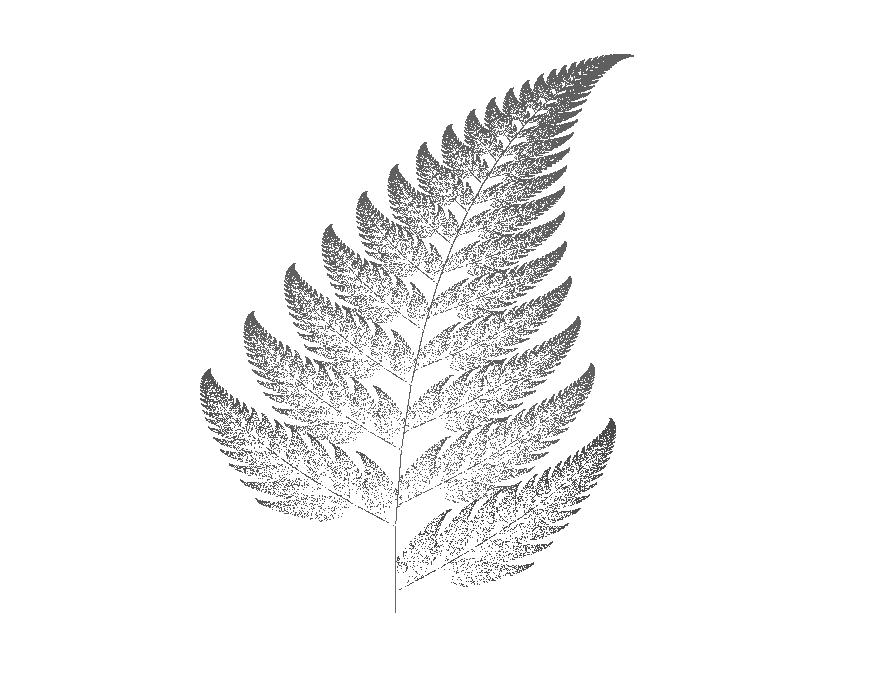
\includegraphics[scale=.5]{images/IFS-fern1.png}
% \includegraphics[scale=.2]{imagesIFS-fern2.png} 
\end{center}
\begin{displaymath}
\begin{array}{c|cccccc}
     & a & b & c & d & e & f \\
\hline
f_1 & 0 & 0 & 0 & 0.16 & 0 & 0 \\
\hline
f_2  & 0.85 &0.04&-0.04&0.85&0&1.6 \\
\hline
f_3 & 0.2 & -0.26 & 0.23 & 0.22 & 0 & 1.6 \\
\hline
f_4  & -0.15 & 0.28 & 0.26 & 0.24 & 0 & 0.44 \\
\end{array}
\end{displaymath}

\bigskip

Voici une explication de chacune des transformations. 
\begin{itemize}
  \item La première transformation $f_1$ est une projection composée avec une homothétie d'un petit rapport. Elle envoie toute la fougère sur la base de la tige (la portion verticale).
  \item La seconde transformation $f_2$ transforme la fougère en la partie supérieure de la fougère (tout sauf les branches droite et gauche les plus basses).
  \item La transformation $f_3$ envoie la fougère sur la branche basse de droite.
  \item La transformation $f_4$ envoie la fougère sur la branche basse de gauche.  
\end{itemize}

%---------------------------------------------------------------
\subsection{L'hippocampe}

Avec seulement deux transformations, on construit déjà des objets fascinants.
Voici un exemple de courbe qui n'est pas sans rappeler un hippocampe.

\begin{center}
 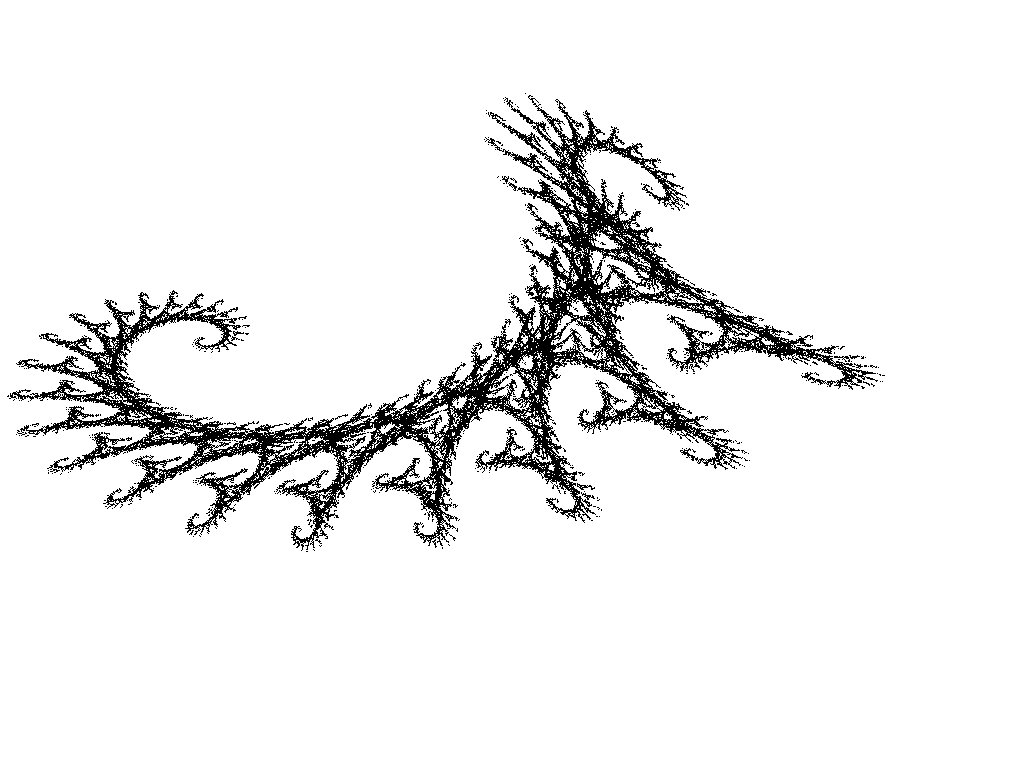
\includegraphics[scale=.5]{images/IFS-dragon1bis.png} 
%\\[2mm]  \includegraphics[scale=.2]{imagesIFS-dragon2.png} 
\end{center}

Les transformations sont :
\begin{displaymath}
\begin{array}{c|cccccc}
     & a & b & c & d & e & f \\
\hline
f_1 & 0.82 & 0.28 & -0.21 & 0.86 & -1.88 & 0.11 \\
\hline
f_2  & 0.88 & 0.52 & 0.46 & -0.37 & 0.78 & 8.09 \\
\end{array}
\end{displaymath}

%---------------------------------------------------------------
\subsection{Vive la géométrie}

Enfin, avec un peu de patience et $12$ transformations (que nous vous laissons le soin de retrouver),
vous pouvez exprimer votre passion pour la géométrie à l'infini !

\begin{center}
 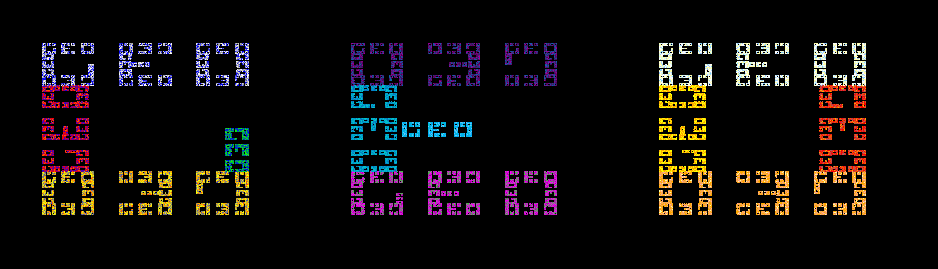
\includegraphics[scale=.5]{images/IFS-geo1.png} \\[2mm]

 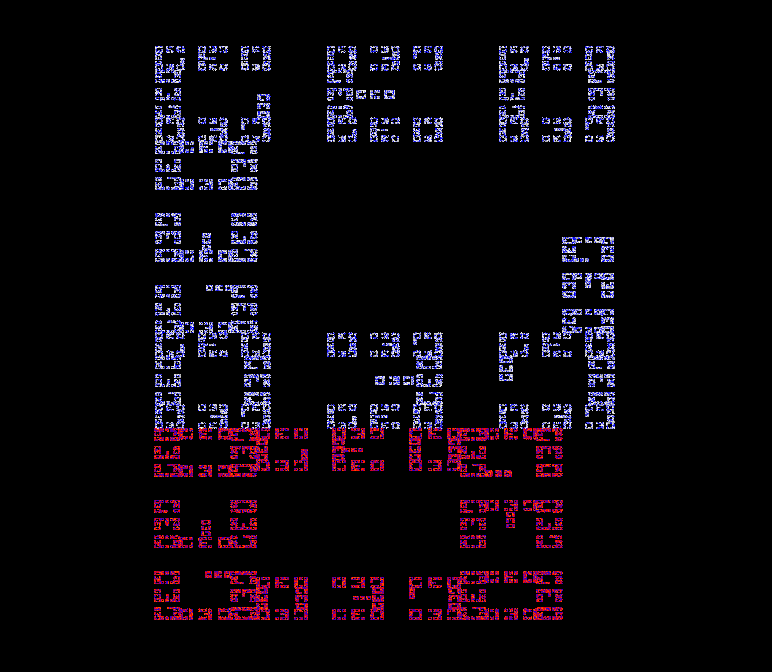
\includegraphics[scale=.2]{images/IFS-geo2.png} 
\end{center}
La seconde image est un zoom du coin supérieur gauche.


%%%%%%%%%%%%%%%%%%%%%%%%%%%%%%%%%%%%%%%%%%%%%%%%%%%%%%%%%%%%%%%%
\section{Dimension de Hausdorff}


%---------------------------------------------------------------
\subsection{Intuition}

Il serait dommage de ne pas parler de dimension d'un ensemble fractal.
Nous allons d'abord comprendre de façon intuitive la notion de dimension.
On doit retrouver que la dimension d'un segment est $1$,
d'un carré est $2$ et d'un cube est $3$.

Prenons l'exemple d'un carré : si on le réduit d'un facteur $m=2$,
alors il faut $\ell=4=m^2$ petits carrés pour reconstituer le carré initial.
L'exposant $2$ est la dimension de la figure du carré plein. Remarquez que si
on décide de réduire notre carré initial d'un facteur $m=3$,
alors $\ell=9=m^2$. On retrouve le même exposant $d=2$.
%\commentfigure{
\myfigure{1}{\tikzinput{fig_ifs16}}
%}


Prenons un cube : si on le réduit d'un facteur $m=2$, il faut 
$\ell=8=m^3$ petits cubes pour reconstituer le cube initial.
Si on le réduit d'un facteur $m=3$, il faut 
$\ell=27=m^3$ petits cubes (voir la figure ci-dessous).
Plus généralement, si on réduit notre cube initial d'un facteur $m$, il faut
$\ell=m^3$ petits cubes. La dimension est l'exposant $d=3$.

%\commentfigure{
\myfigure{1}{\tikzinput{fig_ifs17}}
%}

Pour un segment, si on le réduit d'un facteur $m$, alors on retrouve
$\ell=m^1$ petits segments : la dimension est donc $d=1$.

On voit que la dimension $d$ d'un ensemble $E$ vérifie 
$$\ell=m^d,$$
tel qu'après une réduction d'un facteur $m$, il faut $\ell$ objets 
réduits pour reconstituer l'ensemble initial. 

Nous allons calculer notre première dimension fractale.
Prenons l'exemple du flocon de Koch : 
\commentfigure{
\myfigure{1}{\tikzinput{fig_ifs-koch01}}
}
Après réduction d'un facteur $m=3$ (les contractions sont de rapport $\frac 13$),
il faut $\ell = 4$ ensembles réduits pour reconstituer le flocon.
Donc la dimension du flocon est le réel $d$ tel que $4= 3^d$.
En prenant le logarithme on obtient $\ln 4 = d\cdot \ln 3$ et 
donc $d = \frac{\ln 4}{\ln 3}$.
La dimension (dite de Hausdorff) du flocon de Koch est donc $d=1,2618\ldots$
C'est donc \og plus gros \fg{} qu'une courbe de dimension $1$ mais \og plus petit \fg{} 
qu'une surface de dimension $2$.

Si on reformule ceci à l'aide de notre famille d'itération $\mathbf{f}=\{f_1,f_2,f_3,f_4\}$,
alors chacune est une contraction de rapport $k=\frac 13$ (donc le facteur de réduction est $m=3$)
et on trouve la relation 
$$\ell \cdot k^d = 1$$
avec $\ell=4$, le nombre de fonctions dans notre famille. 





%---------------------------------------------------------------
\subsection{Dimension pour un système itéré de fonctions}

Nous allons énoncer un théorème qui permet de calculer la dimension de Hausdorff
d'un attracteur obtenu pour un certain type de système itéré de fonctions $\mathbf{f}=\{f_i\}$.
Les fonctions considérées sont ici des similitudes contractantes et l'on note $0<k_i<1$
le réel tel que, pour tous $P,Q \in \Rr^2$, 
$$\|f_i(P)-f_i(Q)\| = k_i \|P-Q\|.$$

Il nous faut en plus une \defi{condition de non-recouvrement} : on suppose qu'il existe un ouvert
$O \subset \Rr^2$ tel que $\bigcup_{i=1}^{\ell} f_i(O) \subset O$ et 
tel que $f_i(O)$ et $f_j(O)$ soient disjoints si $i\neq j$.

Voici un \og{}théorème\fg{} qui pour nous sera la définition de la dimension de Hausdorff.
\begin{theoreme}
\sauteligne
\begin{enumerate}
  \item Soit $\mathbf{f}=\{f_i\}_{i=1,\ldots,\ell}$ une famille de similitudes contractantes de rapport $k_i$.
Alors il existe un réel $d>0$ tel
que :
$$\sum_{i=1}^\ell k_i^d =1.$$
  \item Si la condition de non-recouvrement est vérifiée, alors 
  $d$ est la \defi{dimension de Hausdorff} de l'attracteur.
  \end{enumerate}
\end{theoreme}

\bigskip

\textbf{Premier exemple} (en dimension $1$) : l'ensemble de Cantor $C$. 
On rappelle que $f_1(x)=\frac 13x$, 
$f_2(x)=\frac 23 + \frac 13x$.
Les transformations sont
bien des similitudes de rapport $k_1=k_2=\frac13$.
Si l'on prend $O=]0,1[$ (un ouvert de $\Rr$) alors $f_1(O) = ]0,\frac 13[$, 
$f_2(O)=]\frac 23,1[$. 
La condition de non-recouvrement est vérifiée car $f_1(O)\cup f_2(O) \subset O$
et $f_1(O)\cap f_2(O)=\varnothing$.
Nous cherchons donc $d$ tel que :
$$\left(\frac 13 \right)^d + \left(\frac 13 \right)^d =1.$$
Cela revient à l'équation $2= 3^d$ ou encore
$\ln 2 = d \ln 3$ et donc 
$$\dim_H C = \frac{\ln 2}{\ln 3}.$$

La dimension de l'ensemble de Cantor vaut donc environ $0,6309\ldots$


\bigskip

\textbf{Deuxième exemple} : le triangle de Sierpinski $S$.
Les fonctions $f_1, f_2, f_3$ sont des similitudes de rapport
$k_i=\frac 12$. Pour la condition de non-recouvrement, on prend $O$
le triangle ouvert. Le théorème nous donne alors la relation
$$\left(\frac 12 \right)^d + \left(\frac 12 \right)^d+\left(\frac 12 \right)^d = 1.$$
Et donc $\dim_H S = \frac{\ln 3}{\ln 2}.$
Bien sûr, on aurait pu calculer la dimension directement à partir de la définition : après une réduction d'un facteur
$m=2$, il faut $\ell=3$ triangles réduits pour reconstituer le triangle initial, donc la dimension $d$ vérifie $3=2^d$.

%%%%%%%%%%%%%%%%%%%%%%%%%%%%%%%%%%%%%%%%%%%%%%%%%%%%%%%%%%%%%%%%
\section{Le théorème du collage et le jeu du chaos}

%---------------------------------------------------------------
\subsection{Le théorème du collage}


Vu le caractère \og chaotique \fg{} de certaines figures, il est important d'avoir
un résultat qui affirme que nos attracteurs sont stables pour l'unicité : si l'on prend 
un ensemble $E$ qui est proche de $\mathbf{f}(E)$,
alors en fait $E$ est proche de l'attracteur $C$. 


\begin{proposition}
\label{prop:stable}
Soit $\mathbf{f}=\{f_i\}$ une famille de contractions de rapports $k_i \le k <1$.
Soit $C$ l'attracteur de la famille $\mathbf{f}$.
Alors, pour tout compact non vide $E \subset \Rr^2$,
$$\dist_H(E,C) \le \frac{1}{1-k} \dist_H (E,\mathbf{f}(E)).$$
\end{proposition}

\begin{proof}
\begin{align*}
\dist_H(E,C) 
   &\le \dist_H(E,\mathbf{f}(E))+ \dist_H(\mathbf{f}(E),C)\quad \text{ par l'inégalité triangulaire} \\
   &= \dist_H(E,\mathbf{f}(E))+  \dist_H(\mathbf{f}(E),\mathbf{f}(C)) \quad \text{ car } \mathbf{f}(C) = C\\  
   &= \dist_H(E,\mathbf{f}(E))+  k \cdot \dist_H(E,C) \quad \text{ car $\mathbf{f}$ est une famille de contractions}         
\end{align*}
D'où le résultat.               
\end{proof}


Enfin, quelles sont les figures que l'on peut représenter par des attracteurs ?
Réponse : toutes ! La proposition suivante, appelée \og{} théorème du collage\fg{},
affirme que, pour n'importe quelle partie compacte $E$, on peut trouver
une famille de contractions dont l'attracteur $C$ approxime $E$.
\begin{theoreme}[du collage]
Soit $E$ une partie non vide et compacte de $\Rr^2$.
Pour chaque $\epsilon >0$, il existe une famille $\mathbf{f}=\{f_i\}$ de contractions 
ayant pour attracteur un ensemble $C$ tel que 
$$\dist_H(E,C) \le \epsilon.$$
\end{theoreme}

\begin{proof}
Soit $\epsilon >0$. Nous recouvrons notre compact 
$E$ par un nombre fini de disques ouverts $D_1,\ldots,D_\ell$,
chacun de rayon $\frac{\epsilon}{4}$ et dont les centres appartiennent à $E$.
Pour chaque disque $D_i$, nous fixons et notons $f_i$ une contraction de rapport $k_i \le \frac 12$,
telle que $f_i(E)\subset D_i$. Nous notons aussi $C$ l'attracteur de la famille $\mathbf{f}=\{f_i\}$.

Nous allons calculer la distance de Hausdorff entre $E$ et $\mathbf{f}(E)$ pour appliquer
la proposition \ref{prop:stable}.
Pour calculer la distance de Hausdorff, nous montrons deux inclusions.
Pour la première inclusion, comme $f_i(E) \subset D_i$, alors $\mathbf{f}(E)=\bigcup_{i} f_i(E) \subset \bigcup_i D_i
\subset E(\frac{\epsilon}{4})$, où $E(\frac{\epsilon}{4})$ est le $\frac{\epsilon}{4}$-voisinage de $E$.
Pour l'autre inclusion, nous avons $D_i \subset (f_i(E))(\frac \epsilon 2)$ 
(car $D_i$ est de rayon $\frac\epsilon 4$ et $f_i(E) \subset D_i$).
%[[dessin]]
Donc $E \subset \bigcup_i D_i \subset \bigcup_i (f_i(E))(\frac \epsilon 2) = \mathbf{f}(E)(\frac\epsilon 2)$.
Donc $\dist_H(E,\mathbf{f}(E)) \le \frac \epsilon 2$, et nous appliquons alors
la proposition \ref{prop:stable} (avec $k=\frac12$) pour en déduire $\dist_H(E,C) \le \epsilon$.
\end{proof}

\bigskip

Au début de la preuve, nous avons implicitement utilisé le théorème suivant sur les compacts.
\begin{theoreme}
Soit $C \subset \Rr^2$ un compact.
Si on a un recouvrement de $C$ par des disques ouverts, alors on peut en extraire un recouvrement fini. 
\end{theoreme}
Nous l'avons appliqué de la façon suivante :
pour chaque $P \in C$, on considère le disque $D_P$ centré en $P$ et de rayon $r$ 
(ici $r$ était $\epsilon/4$). Alors on a bien un recouvrement de $C$ par tous les disques $D_P$ :
$C \subset \bigcup_{P\in C} D_P$. Le théorème nous affirme que, parmi tous ces disques, un nombre fini est suffisant.
Donc il existe des points $P_1,\ldots, P_\ell$ tels que $C \subset \bigcup_{i=1,\ldots,\ell} D_{P_i}$.


%---------------------------------------------------------------
\subsection{Le jeu du chaos}
\label{ssec:chaos}

Comment en partant d'un seul point, choisi au hasard, peut-on tracer l'attracteur de n'importe quel système itéré de fonctions ?

Soit $P_0$ un point quelconque de $\Rr^2$. Notons
$E = \{ P_0 \}$, puis $E_1 = \mathbf{f}(E) = \{f_1(P_0),\ldots,f_\ell(P_0)\}$,
et de façon générale $E_j = \mathbf{f}^j(E)$. 
Le théorème \ref{th:attractionbis} prouve alors que 
$\mathbf{f}^k(E)$ tend vers l'attracteur $C$. Autrement dit, en prenant l'union de $E_j$ avec 
des $j$ assez grands, on approche l'attracteur.

\bigskip

La façon la plus efficace de tracer un attracteur à l'aide d'un ordinateur est alors la suivante, 
appelée \og{} jeu du chaos \fg{} :
partant d'un point quelconque $P_0 \in \Rr^2$, on construit une suite de points par récurrence.
Si $P_k$ est construit, alors on choisit aléatoirement l'une des transformations
$f_i$ de la famille $\mathbf{f}$ et on définit $P_{k+1}=f_i(P_k)$. 
On laisse de côté les premiers points (disons les $100$ premiers qui peuvent être \og loin \fg{} de l'attracteur) et on trace les points suivants : ces points sont des éléments très proches de l'attracteur
et en en traçant suffisamment, ils représentent tout l'attracteur.

La proposition \ref{prop:stable} explique aussi que les calculs numériques (et donc approchés) 
des ordinateurs sont justifiés. 

\bigskip


\textbf{Algorithme \og jeu du chaos \fg{}.}

\textbf{Entrée :} une famille $\mathbf{f} = \{ f_i\}_{i=1,\ldots,\ell}$ de contractions.

\textbf{Sortie :} un tracé approché de l'attracteur.

\begin{itemize}
  \item Fixer $P_0 \in \Rr^2$ au hasard.
    
  \item Pour $k \in \{0,\ldots,N_{\max}\}$ :
  \begin{itemize}
      \item on choisit au hasard $i \in \{1,\ldots,\ell\}$,
      \item on pose $P_{k+1} = f_i(P_k)$,
      \item à partir de $k \ge N_{\min}$ on affiche ce point.
  \end{itemize}
\end{itemize}

\bigskip

$N_{\max}$ représente le nombre de points à calculer (par exemple $N_{\max} = 10\,000$).
$N_{\min}$ est une constante (par exemple $N_{\min} = 100$) qui permet de ne pas tracer les tout premiers points
qui peuvent être loin de l'attracteur.


En plus, pour optimiser les calculs, on ne choisit pas les transformations $f_i$ de façon équiprobable mais 
avec une probabilité $p_i$. Cette probabilité $p_i$ correspond à la surface couverte par $f_i(C)$ par rapport à celle couverte par $C$. Voici les probabilités pour la fougère de Barnsley : par exemple, la transformation
$f_1$ qui correspond à un bout de la tige n'est choisie que dans $1\%$ des cas, alors que la transformation
$f_2$ est choisie dans $85\%$ des cas...


\begin{displaymath}
\begin{array}{c|ccccccc}
     & a & b & c & d & e & f & p\\
\hline
f_1 & 0 & 0 & 0 & 0.16 & 0 & 0 & 0.01\\
\hline
f_2  & 0.85 &0.04&-0.04&0.85&0&1.6 & 0.85 \\
\hline
f_3 & 0.2 & -0.26 & 0.23 & 0.22 & 0 & 1.6 & 0.07 \\
\hline
f_4  & -0.15 & 0.28 & 0.26 & 0.24 & 0 & 0.44 & 0.07 \\
\end{array}
\end{displaymath}

\medskip

C'est avec cette méthode qu'a été tracée la fougère de Barnsley, dont voici un zoom.

\begin{center}
 %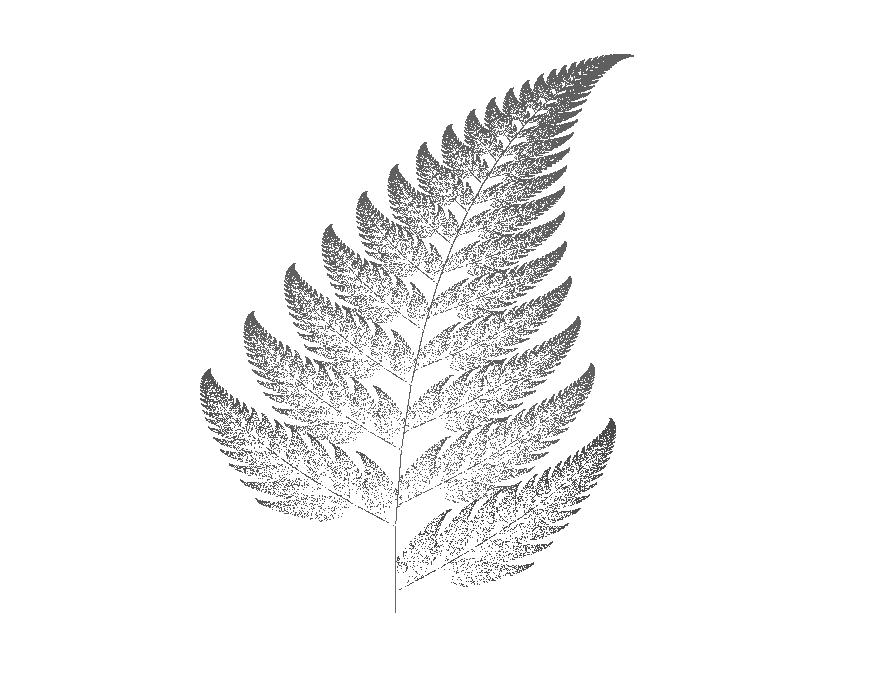
\includegraphics[scale=.5]{images/IFS-fern1.png} \\[2mm]
 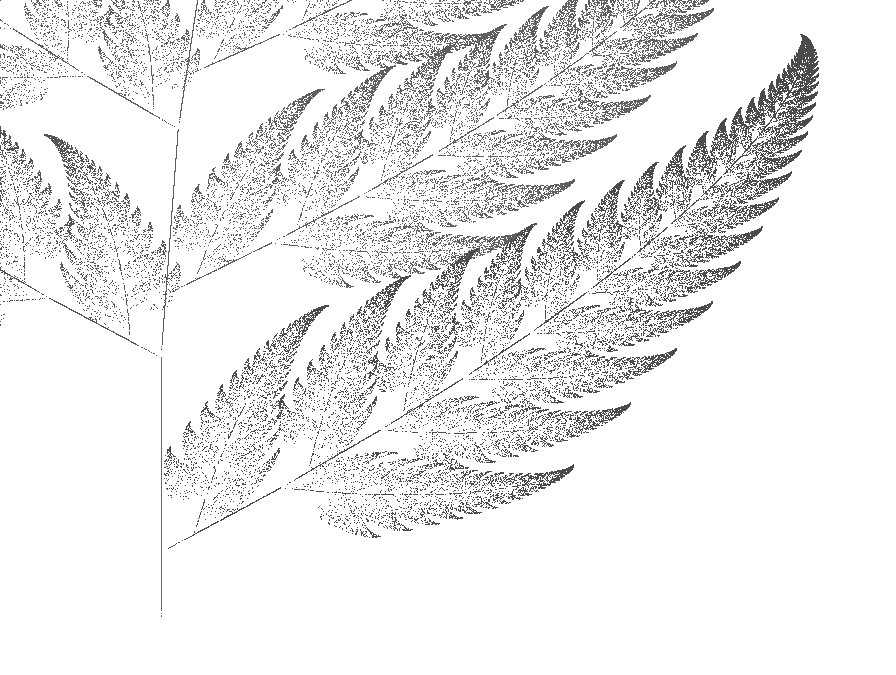
\includegraphics[scale=.2]{images/IFS-fern2.png} 
\end{center}



%%%%%%%%%%%%%%%%%%%%%%%%%%%%%%%%%%%%%%%%%%%%%%%%%%%%%%%%%%%%%%%%
\section{Exercices}

% Autres idées : la courbe du dragon/pliage du papier

%%%%%%%%%%%%%%%%%%%%%%%%%%%%%%%%%%%%%%%%%%%%%%%%%%%%%%%%%%%%%%%%
\subsection{Le flocon de Koch}

\begin{exercicecours}[Flocon de Koch]
$K_0$ est un triangle équilatéral, chaque côté étant de longueur $1$.
$K_n$ désigne la $n$-ème étape dans la construction du flocon de Koch. 
\begin{enumerate}
 \item Calculer la longueur de la courbe $K_n$.
 \item Calculer l'aire de la surface délimitée par $K_n$.
 \item Quelle est la longueur et la surface du flocon de Koch (la limite de $K_n$) ?
\end{enumerate}

\commentfigure{
\myfigure{1}{\tikzinput{fig_ifs-koch05}}
}
\end{exercicecours}


%%%%%%%%%%%%%%%%%%%%%%%%%%%%%%%%%%%%%%%%%%%%%%%%%%%%%%%%%%%%%%%%
\subsection{Topologie de $\Rr^2$}



\begin{exercicecours}[Distance de Hausdorff]
\label{exo:ifs2}
\sauteligne
\begin{enumerate}
  \item  Dessiner, pour différentes valeurs de $r>0$, les $r$-voisinages d'un carré, d'un carré plein, d'un cercle, d'un disque.
  
  \item Montrer que pour tout ensemble $E$ et pour tous $r,r' \ge 0$ : $E(r)(r')=E(r+r')$.

 \item Calculer $\dist_H (E,F)$ dans chacun des cas suivants :
  \begin{enumerate}
     \item $E$ est le cercle de rayon $1$ centré à l'origine, $F$ est le disque de rayon $1$ centré à l'origine.

     \item $E$ est le carré de côté de longueur $1$ centré à l'origine, $F$ est le cercle de rayon $R$ centré à l'origine. Quel cercle approche le mieux le carré ?

     \item $E=K_n$, $F=K_{n+1}$, où les $K_i$ sont les itérations conduisant au flocon de Koch.
  \end{enumerate}
 \item Montrer que la distance de Hausdorff $\dist_H$ vérifie l'inégalité triangulaire.
 \item Monter que, si $C, C'$ sont deux compacts de $\Rr^2$ et $f$ est une application
$k$-contractante, alors $\dist_H (f(C),f(C')) \le k \cdot \dist_H (C,C')$.

\end{enumerate}
\end{exercicecours}


\begin{exercicecours}[Ensemble de Cantor]


Soit l'ensemble de Cantor $C$ obtenu en itérant le processus suivant.
On divise l'intervalle $C_0 = [0,1]$ en trois intervalles, on retire l'intervalle central pour obtenir 
$C_1=[0,\frac13] \cup [\frac 23,1]$. On obtient $C_2$ en retirant l'intervalle central de chacun des sous-intervalles de $C_1$,\ldots
Par définition, $C = \bigcap_{n\ge0} C_n$.
\begin{enumerate}
  \item Calculer la somme des longueurs des sous-intervalles de $C_n$.
  \item Montrer que $C$ est un compact.
  \item Montrer que $C$ est d'intérieur vide : si $x,x' \in C$ (avec $x<x'$) alors il existe$y \in [x,x']$ tel que $y\notin C$.
  \item Montrer que $x\in C$ si, et seulement si, il admet une écriture en base $3$ ne contenant que des $0$ et des $2$ :
$$x = \sum_{n=0}^{+\infty} \frac{a_n}{3^n},\qquad a_n\in \{0,2\}.$$
  \item Montrer que $C$ n'est pas un ensemble dénombrable.
\end{enumerate}

\commentfigure{
\myfigure{1}{\tikzinput{fig_ifs-cantor02}}
}



\end{exercicecours}



%%%%%%%%%%%%%%%%%%%%%%%%%%%%%%%%%%%%%%%%%%%%%%%%%%%%%%%%%%%%%%%%
\subsection{Isométries, similitudes, transformations affines}


\begin{exercicecours}
\sauteligne
\begin{enumerate}
 \item Expliciter deux isométries $f,g$ telles que $f\circ g$ et $g\circ f$ soient distinctes.
  \item Montrer qu'une similitude directe d'angle $\theta$ et de rapport $k$ composée 
avec une similitude directe d'angle $\theta'$ et de rapport $k'$
est une similitude directe d'angle $\theta+\theta'$ et de rapport $k\cdot k'$. 
 \item Montrer que l'ensemble des similitudes directes forme un groupe pour la composition.
\end{enumerate}
\end{exercicecours}


\begin{exercicecours}
Dessiner l'image du Shadok représenté ci-dessous par chacune des transformations
$$\myvec{x}{y} \mapsto \begin{pmatrix}a & b \\ c & d \\  \end{pmatrix}
\myvec{x}{y} + \myvec{e}{f}$$

\commentfigure{
\myfigure{1}{\tikzinput{fig_ifs_exo05}}
}


Avec :
\begin{enumerate}
 \item $a=\sqrt 3$, $b=-1$, $c=1$, $d=\sqrt 3$, $e=-4$, $f=0$.
 \item $a=\frac 12$, $b=1$, $c=0$, $d=1$, $e=3$, $f=0$.
 \item $a=3$, $b=-1$, $c=-2$, $d=-1$, $e=-2$, $f=1$.
\end{enumerate}
\end{exercicecours}


\begin{exercicecours}
Quelles sont les transformations affines qui envoient le Shadok centré sur l'axe des ordonnées sur l'autre Shadok ?
\begin{center}
\commentfigure{
\myfigure{1}{\tikzinput{fig_ifs_exo01}}
\myfigure{1}{\tikzinput{fig_ifs_exo02}}
}
\end{center}

\begin{center}
\commentfigure{
\myfigure{1}{\tikzinput{fig_ifs_exo03}}
%[cm={2,1,1,2,(4,2)}]
\myfigure{1}{\tikzinput{fig_ifs_exo04}}
%[cm={-2,-1,-0.333,-1,(4,1)}]
}
\end{center}
\end{exercicecours}



%%%%%%%%%%%%%%%%%%%%%%%%%%%%%%%%%%%%%%%%%%%%%%%%%%%%%%%%%%%%%%%%
\subsection{Attracteurs}

\begin{exercicecours}
Trouver les transformations affines permettant de générer ces fractales :
\begin{enumerate}
 \item L'arbre de Cayley (partir d'un carré, le diviser en $9$, n'en garder que $5$ ; il y a $5$ transformations).
 \item Le faux flocon de Koch.
 \item La courbe du dragon.
\end{enumerate}

\begin{center}
\commentfigure{
\myfigure{1}{\tikzinput{fig_ifs-cayley01}}
}
\end{center}

\begin{center}
\commentfigure{
\myfigure{1}{\tikzinput{fig_ifs-badkoch01}}
}
\end{center}

\begin{center}
\commentfigure{
\myfigure{1}{\tikzinput{fig_ifs-dragon01}}
}
\end{center}
\end{exercicecours}


\begin{exercicecours}[\'Enigme]
Quel est l'attracteur correspondant à ces deux premières étapes ?
\begin{center}
\commentfigure{
\myfigure{1}{\tikzinput{fig_ifs-badsierp01}}
}
\end{center}

% Les contractions sont
% $f_1$, homothétie de rapport $k=0.5$ avec translation $(0,0)$, $f_2$, $k=0.5$, avec translation $(0.5,0)$,
% $f_3$, $k=0.5$, avec translation $(0,0.5)$.
% c'est donc bien le triangle de Sierpinski (unicité de l'attracteur).
% Dessins à décommenter dans la figure
\end{exercicecours}



%%%%%%%%%%%%%%%%%%%%%%%%%%%%%%%%%%%%%%%%%%%%%%%%%%%%%%%%%%%%%%%%
\subsection{Dimension de Hausdorff et théorème du collage}

\begin{exercicecours}[Dimension de Hausdorff]
Calculer, lorsque c'est possible, la dimension de Hausdorff de chacun des attracteurs
des exercices de cette fin de chapitre.
\end{exercicecours}


\begin{exercicecours}[\`A l'infini]
Calculer le système de fonctions permettant de dessiner la fractale composée des trois premières lettres
de votre prénom.
\end{exercicecours}


\bigskip
\bigskip

Bilbliographie (en anglais) : Kenneth Falconer, \emph{Fractal Geometry}, 1990, John Wiley \& Sons.

\auteurs{
Arnaud Bodin

Relu par Vianney Combet et Volker Mayer}

\finchapitre
\end{document}


